\documentclass{article}
\usepackage{graphicx}
\usepackage{amsmath}
\usepackage{amssymb}

\title{Leveraging Mathematical Structure in Software Synthesis}
\author{Andr\'{e}s Goens}
\begin{document}
\date{}
\maketitle
\begin{abstract}
The trend is clear: Computing systems of the future will consist of heterogeneous multicores. While this allows for maximal computational efficiency, these systems are extremely difficult to program.
A family of methods that is commonly used to program heterogeneous multicore systems is called \emph{software synthesis}.
It consists of using an abstract representation of the application, which allows to analyze and determine an optimal execution, leveraging heterogeneous resources.
The software synthesis problem has many different subproblems, pertaining the representation of applications and architectures, the recording the behavior of an execution and deciding how to best execute a particular application in an architecture.
Each of these subproblems exhibits much structure, which can be captured in precise mathematical terms. In this thesis we aim to identify, describe and leverage this mathematical structure in different subproblems of the software synthesis process.
This would allow to improve the programmability of heterogeneous multicores, bridging the productivity gap for developers.

\end{abstract}

%\tableofcontents

\section*{Introduction}
%End of moore's law:
Since the invention of the semiconductor, the capacity and performance of computing systems has enjoyed a nearly exponential growth over time. Historically, it has doubled roughly every $1 1/2$ years, an observation which is commonly associated with Moore \cite{schaller1997moore}.
While this trend continues roughly until today, in terms of the number of semiconductors in a computer, the capacity and speed of computing systems has been unable to keep up. It is likely that we are reaching more fundamental barriers, where the laws of physics prevent our
current methods to produce event faster systems. 

%Trend: heterogeneous multicores
Fortunately, we still seem far from reaching the limits of our own ingenuity. In terms of hardware, the trend is clear: The computing systems of the future will consist of heterogeneous multicores. Multicores allow to leverage the technological advances in semiconductors to 
increase the computing power of systems by exploiting parallelism in computation. The heterogeneity of said systems, on the other hand, allows to design units specialized for a particular type of processing, instead of relying solely on general-purpose processors.
While this specialization can have a tremendous impact in the computation speed for some problems, it usually has an even greater impact on energy efficiency, which is arguably even more valuable today.


%problem: programming heterogeneous multicores?
With novel systems come novel problems. While heterogeneous multicores are, in principle, an ideal solution to the complex requirements of today's applications, they come with an equally exceptional challenge.
Programming heterogeneous multicores is difficult. It involves partitioning the required computation into appropriate steps. These steps, in turn, might execute differently well in the various hardware resources on the system,
which might itself depend on the concrete data being processed.
On the other hand, systems incur in significant time and energy costs by transfering data between resources.
To efficiently execute a calculation thus involves orchestrating which steps to execute when and where, a highly non-trivial problem which completely dissapears in the traditional, single-core case.

%a solution: software synthesis
Several approaches have been put forward to deal with these issues.
In particular, a family of promising methods that is commonly used to program heterogeneous multicore systems is called \emph{software synthesis}\cite{bhattacharyya2012software,sgroi1999synthesis}.
It consists of using an abstract, functional representation to describe the application, commonly in the form of a graph. Using this representation,
decisions for mapping the different parts of the application to resources in the architecture, as well as scheduling the execution are taken. These decisions commonly involve static strategies,
but can also include dynamic decisions at run-time. Finally, code is generated using these decisions, such that it might leverage the heterogeneous resources in the architecture.

%many sub-problems in software synthesis: code partitioning/representation of algorithms, tracing/trace analysis, mapping/scheduling, code generation
This software synthesis process, thus, involves several different sub-problems that have to be solved.
The question of how to partition an application and represent it abstractly, particularly, in form of a graph that represents logical dependencies in the application, is a highly non-trivial one.
Assuming such a graph representation, the behavior of the application has to be analyzed.
A general analysis would require, among others, solving the halting problem.
Thus, many common approaches make do with a trace-based approach, where the analysis is restricted to a particular execution, or a set of executions.
Finally, the decision problems of mapping and scheduling involve the knowledge gained from the sub-problems above to consider an exponentially growing number of possibilities and selecting a near-optimal one.

%Problems have mathematical structure! Graph structure of code, traces: monoid, redundancy,  mapping/scheduling (e.g. symmetries, distances)
By virtue of their inherent properties, these problems exhibit a large amount of structure, which can be described and exploited with precise mathematical structures.
The simplest example is the abstract representation of applications.
Using the mathematical structure of directed graphs, properties of the application can be deduced from graph-theoretic principles and graph algorithms can be leveraged for efficiently analyzing these abstract representations of applications.
Similarly, the sets of execution traces of an application can be considered as part of a monoid, usually called the trace monoid. They also have information-theoretic properties that correspond to the relationship between the application and its trace.
The space of mappings, on the other hand, while it grows exponentially, also exhibits much structure. Symmetries in the architecture and application induce symmetries in the mapping space, which can effectively reduce the amount of possibilities to be explored.

%thesis: identify and leverage this mathematical structure to improve software synthesis!
In order to feasibly solve the problems arising in software synthesis and program the heterogeneous manycores with their ever-growing complexity, we must identify and exploit these mathematical structures. The goal of this thesis is to identify and precisely describe 
the mathematical structure in the different subproblems in software synthesis. Then, using the identified structure, we will propose improvements to the state-of-the-art solution methods in order to leverage the mathematical structure inherent in the problems.


\section{The Software Synthesis Problem}

%General software synthesis too broad: concentrate
The term software synthesis covers several different concrete problems, with different abstract representations of applications or architectures.
While the aim of this thesis is to keep the approaches as general as possible, to cover as many variants as possible, concrete instances still have to be considered.
In the following, we will describe the software synthesis problem for executing Kahn Process Networks~\cite{kahn74} in heterogeneous architectures, as described in~\cite{castrillon_springer}.
While this is not the most general instance of software synthesis, it provides enough generality to understand most concepts, while serving as a concrete instance to implement and test the improvements on real examples.
Throughout the thesis we will use this instance as the basis for the software synthesis problem, and will explicitly discuss, when generality is possible, how this is the case and how to leverage it.

\subsection{Kahn Process Networks}

The problem of mapping KPN applications to heterogeneous hardware involves abstractions at different levels, as depicted in Figure~\ref{fig:problem}.
At the \textbf{application} level, programs are described using the KPN model. In this model, applications are partitioned into
different \emph{processes}, which encapsulate the different parts of the computation. These processes are not isolated;
they communicate by exchanging data. In the KPN model this is abstracted by defining communication \emph{channels}
between processes that act as unbounded FIFO buffers. The Kahn \emph{process network} is the resulting system, usually formalized as a graph 
with processes as nodes and channels as edges.

 \begin{figure}
 	\centering
 	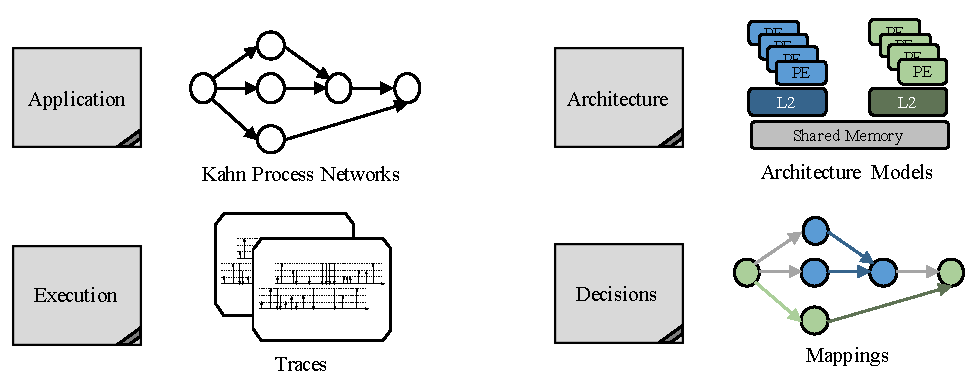
\includegraphics[width=.48\textwidth]{figures/problem.pdf} 
 	%	\vspace{-5mm}
 	\caption{An instance of software synthesis: Mapping KPN applications to heterogeneous architectures.}
 	\label{fig:problem}
 		\vspace{-3mm}
 \end{figure}

The structure offered by KPNs has several advantages. One of these comes at the \textbf{execution} level. 
From its semantics, KPN applications are deterministic~\cite{kahn74}. 
That is, the process network will always produce the same results given the same input.
In particular, the results are independent of the execution order of the processes and individual timings,
provided no artificial deadlocks are introduced when restricting the sizes of the FIFO buffers.
This fact can be utilized to create program traces of a KPN application that are independent of the execution,
capturing the behavior of the execution at a high abstraction level.

Abstractions are also required for describing the hardware \textbf{architecture}.
To this end, an architecture is described as a set of \emph{processing elements} (PEs) and \emph{communication resources}.
The latter is an abstraction for any way data can be shared between processes residing on one or several PEs. 
These range from simply shared memories, and local scratchpads for single PEs, to specialized resources like hardware-FIFOs.
Actual hardware architectures, and the libraries used (or operating system, if applicable), are much more complex than this.
However, there is no simple abstraction that allows to capture all these details in a straightforward manner, 
which is why different frameworks use different such abstractions.

Using these models, \textbf{decisions} are made for deploying the applications onto the hardware. At this level,
one also uses abstractions. As is canonical from the application description, processes are mapped to PEs, 
and the communication channels between them to hardware resources. It is also common to distinguish between the mapping of
processes to PEs and the scheduling at runtime.
In this thesis, we limit ourselves to scheduling within a single PE when several processes have been mapped to it.
There are additional decisions that have to be taken in this context, like \emph{buffer sizing}, where the sizes of the
FIFO buffers have to be chosen. 

The problem of mapping KPN applications to heterogenous hardware, as studied in this thesis, is that of
finding a mapping of processes to PEs and of channels to communication resources. 
This mapping should be optimal or at least near-optimal in some sense for a particular execution, which is captured in the form of a trace.
Optimality can be defined in different ways, like execution time, energy consumption or resource usage (while respecting a particular real-time bound).

A concrete implementation aimed at solving this precise problem is realized in the commercial software suite SLX, which is based on the MAPS framework~\cite{castrillon_maps,castrillon_springer}
The application is written as a KPN in an extension to the C programming language, CPN~\cite{ceng_cpn}. Similarly, an architecture description is given as an xml file.
The tool uses novel methods for performance estimation to extrapolate the performance of the execution in the target architecture~\cite{eusse}, generate a mapping with heuristics~\cite{castrillon_dac12,castrillon_industrial_informatics} and produce executable code.
This thesis will use SLX tools to evaluate approaches and improvements, whenever applicable.

Figure~\ref{fig:synthesisflow} shows an abstract representation of the software synthesis flow, as described above and implemented in SLX.
\begin{figure}[h]
	\centering
	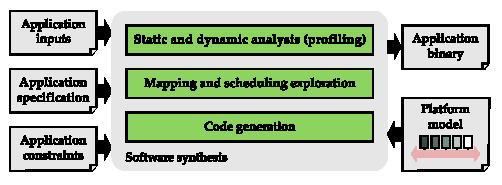
\includegraphics[width=0.60\textwidth]{figures/synthesisflow.pdf}
	\caption{Abstract view of a software synthesis flow}
	\label{fig:synthesisflow}
\end{figure}


\section{Current Status}

In the following section we will describe our previous work leveraging mathematical structure in software synthesis. For space reasons, this exposé cannot go in-depth in the mathematical structures and the methods devised to leverage them.
Instead, the aim of this section is to give an overview and present results, to show how, in principle, mathematical structure can be leveraged to improve solutions to the software synthesis problem.

\subsection{Symmetry in mappings}

The mapping of applications described by an abstract, graph-based representation to heterogeneous architectures exhibits many symmetries, in practice~\cite{goens_iess,goens_taco}. Consider the example shown in Figure~\ref{fig:symmetries_idea}.
To illustrate the principle, the figure depicts a simple homogeneous many-core with a network-on-chip interconnect. Due to the homogeneous structures of the platform, it is intuitive to see that the two leftmost mappings of tasks to processing nodes should lead to basically the same execution behavior, 
if we neglect effects like process variation or aging.
Conversely, we can expect the third, rightmost mapping to have a different execution behavior, since the communication paths are different than in the first two. 
In the presence of heterogeneous resources, such an analysis becomes less obvious.
Even more so with complex network topologies, in architectures with hierarchical structure, when optimizing for different objectives, or when all these are combined.
\begin{figure}[h]
	\centering
	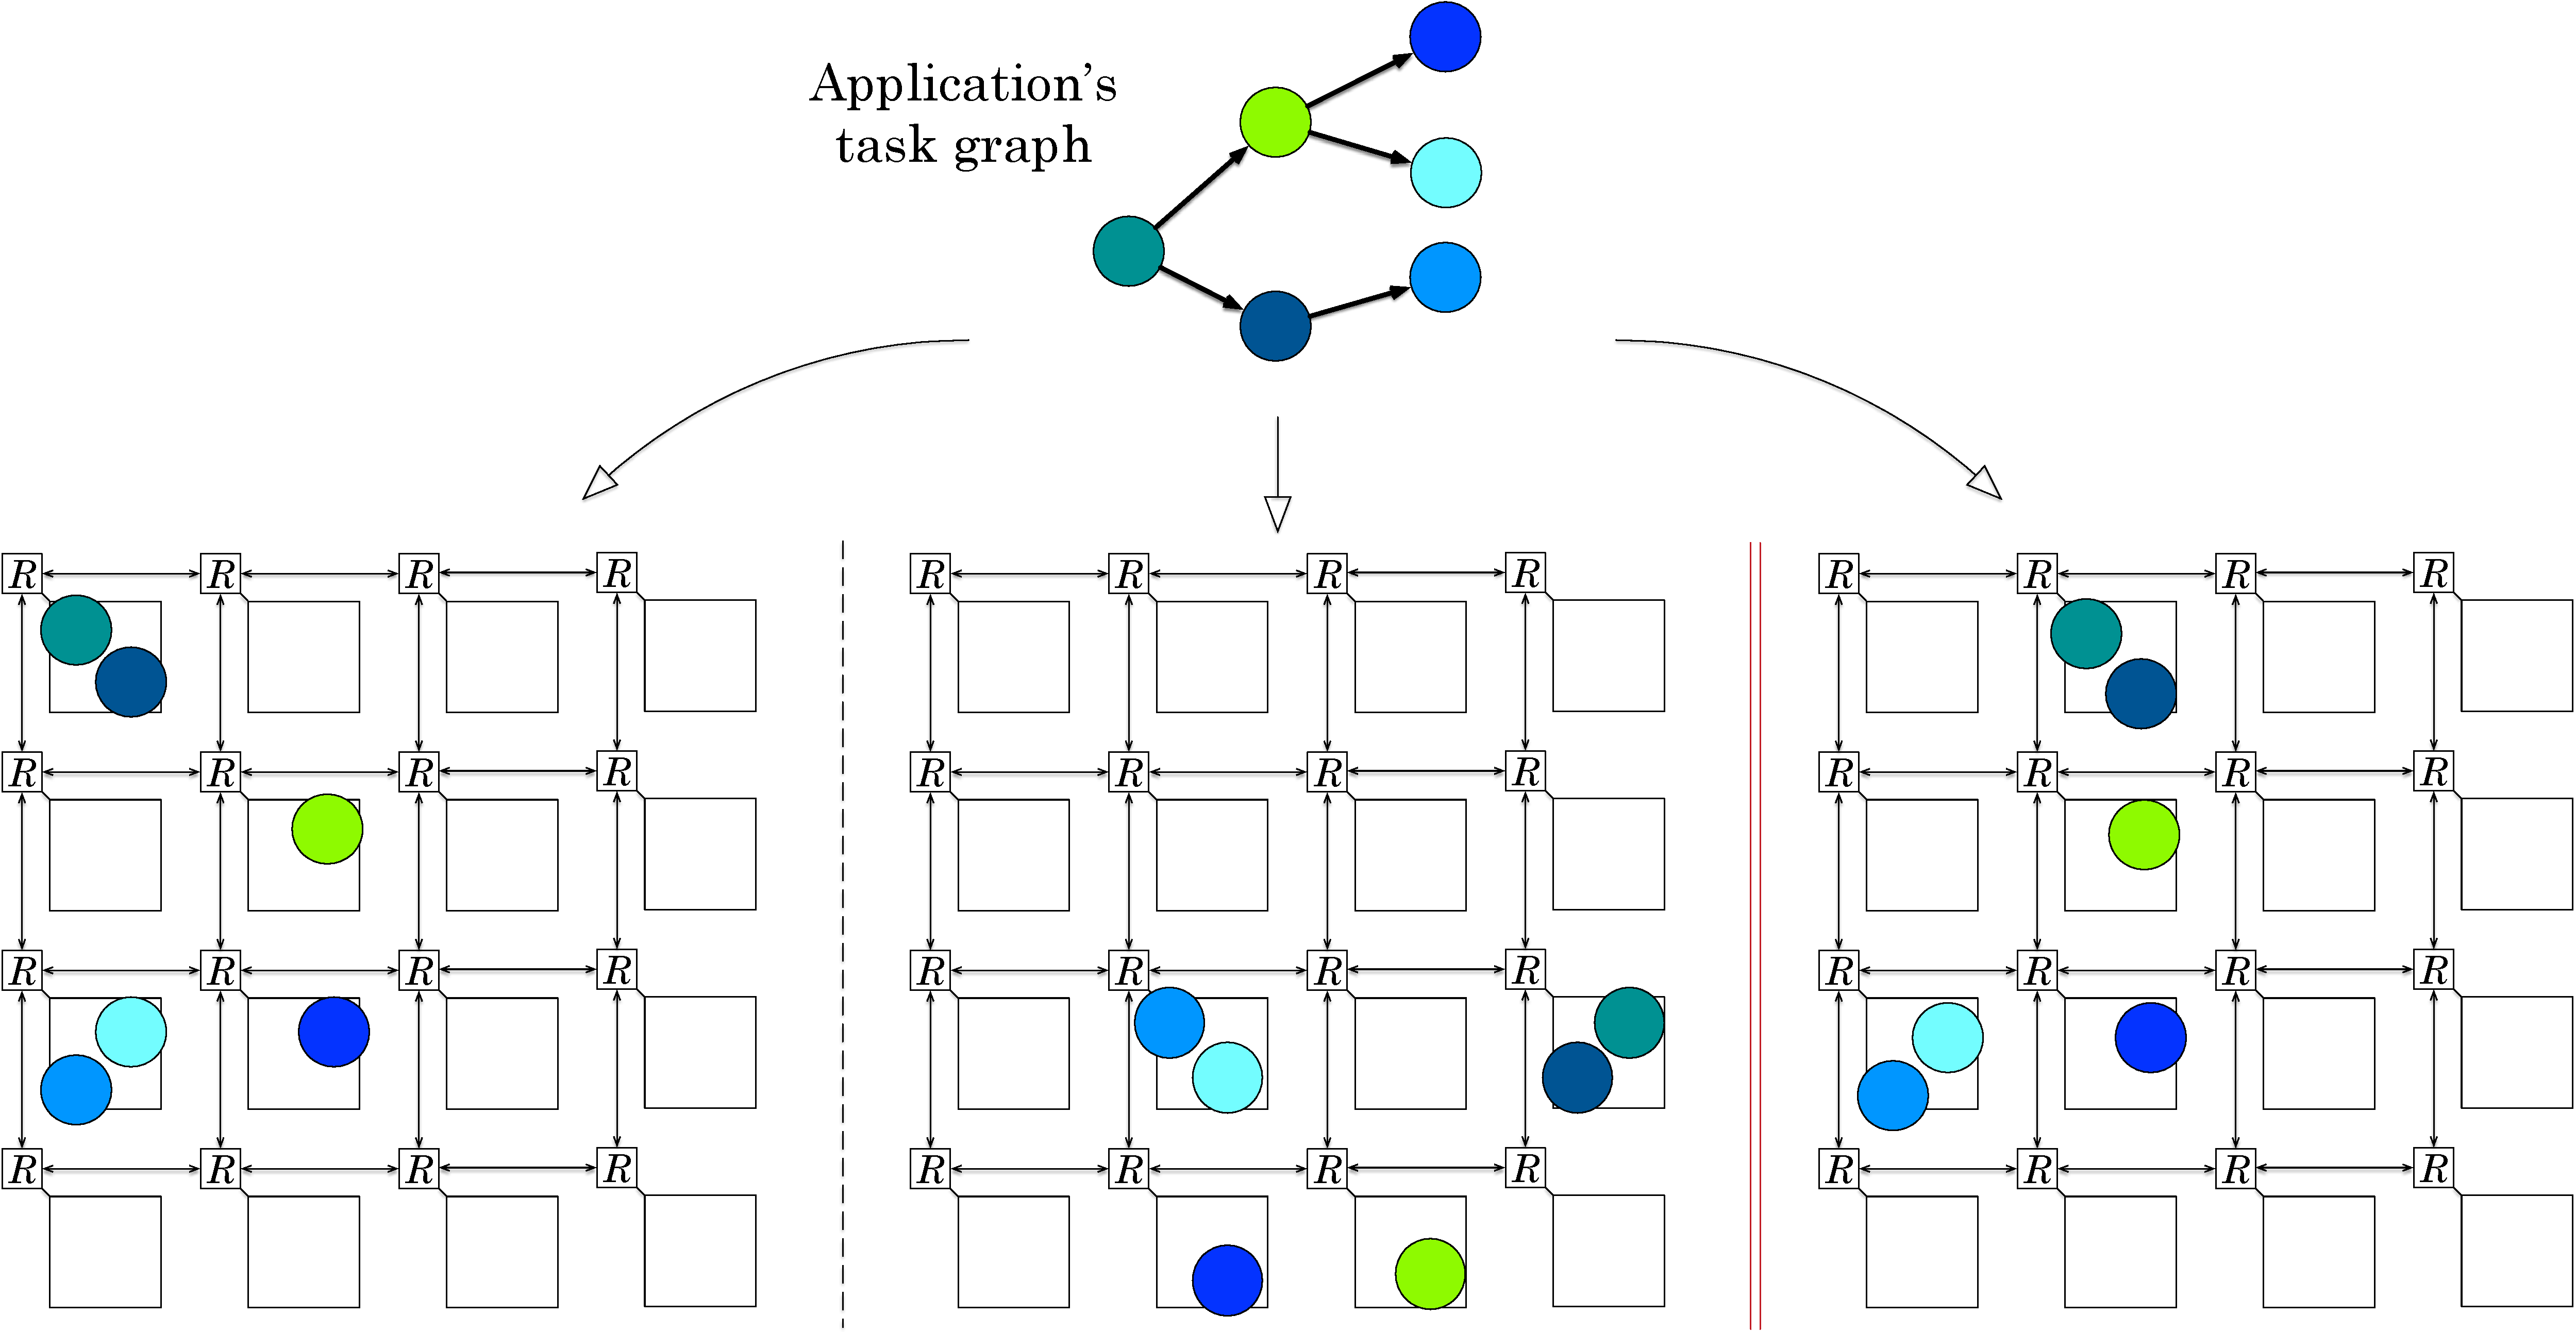
\includegraphics[width=0.65\textwidth]{figures/SymmetriesIntro.pdf}
	\caption{Illustration of symmetries. The two left mappings are equivalent, while the one on the right is not.}
	\label{fig:symmintro}
\end{figure}


\subsubsection{Mathematical Structures}

In order to describe mappings of KPNs to heterogeneous architectures mathematically, we need a mathematical description of the architecture and of the KPN. 
A KPN has a very precise mathematical definition, for its semantics, as can be found in the original paper by Gilles Kahn~\cite{kahn74}. However, for this exposé the semantics are not essential. Thus, it suffices to consider them as a directed
graph $K = (V_K,E_K)$ with a vertex set $V_K$ of processes, and an edge set $E_K$ of channels. Processes can execute concurrently and communicate solely through the channels, which can be though of as FIFO buffers.

For describing architectures, our approach uses a structure called the \emph{architecture graph} to capture the architecture topology~\cite{castrillon2012}. This multigraph $A = (V_A, E_A)$ has a node $v \in V_A$ for every processing element (PE) in the architecture.
A function $l$ labels all the PEs in $V_A$ with their PE type in heterogeneous architectures.

For every communication resource $r$ that can be used between two PEs $v_1, v_2 \in V_A$, the architecture graph has an edge $(v_1,v_2,r) \in E_A$, where $r$ is a label for that communication resource.
As an example, consider the Exynos architecture, as illustrated in Figure~\ref{fig:exynos}.
It has eight ARM PEs, following the big.LITTLE\texttrademark~principle, with four ARM Cortex A7 PEs (the ``little'' ones) and four ARM Cortex A15 PEs (the ``big'' ones). 
For it, the architecture graph of the Exynos architecture is depicted in Figure~\ref{fig:arch_graph}. The labels for the different communication resources and PE types can be seen in the colors of the edges and nodes in the graph.

This architecture graph can be readily obtained from the architecture description in the SLX Tool Suite, or any similar description which includes the structure of the hardware architecture. 
In fact, the objective of the architecture graph is to allow us to capture, in a mathematical object, precisely this \textbf{structure}: the topology, PE types and the communication resources available.
Only by using the formal nature of this architecture graph we can extract the symmetries of the architecture algorithmically, i.e., in an automated fashion.

\begin{figure}[t]
	\centering
	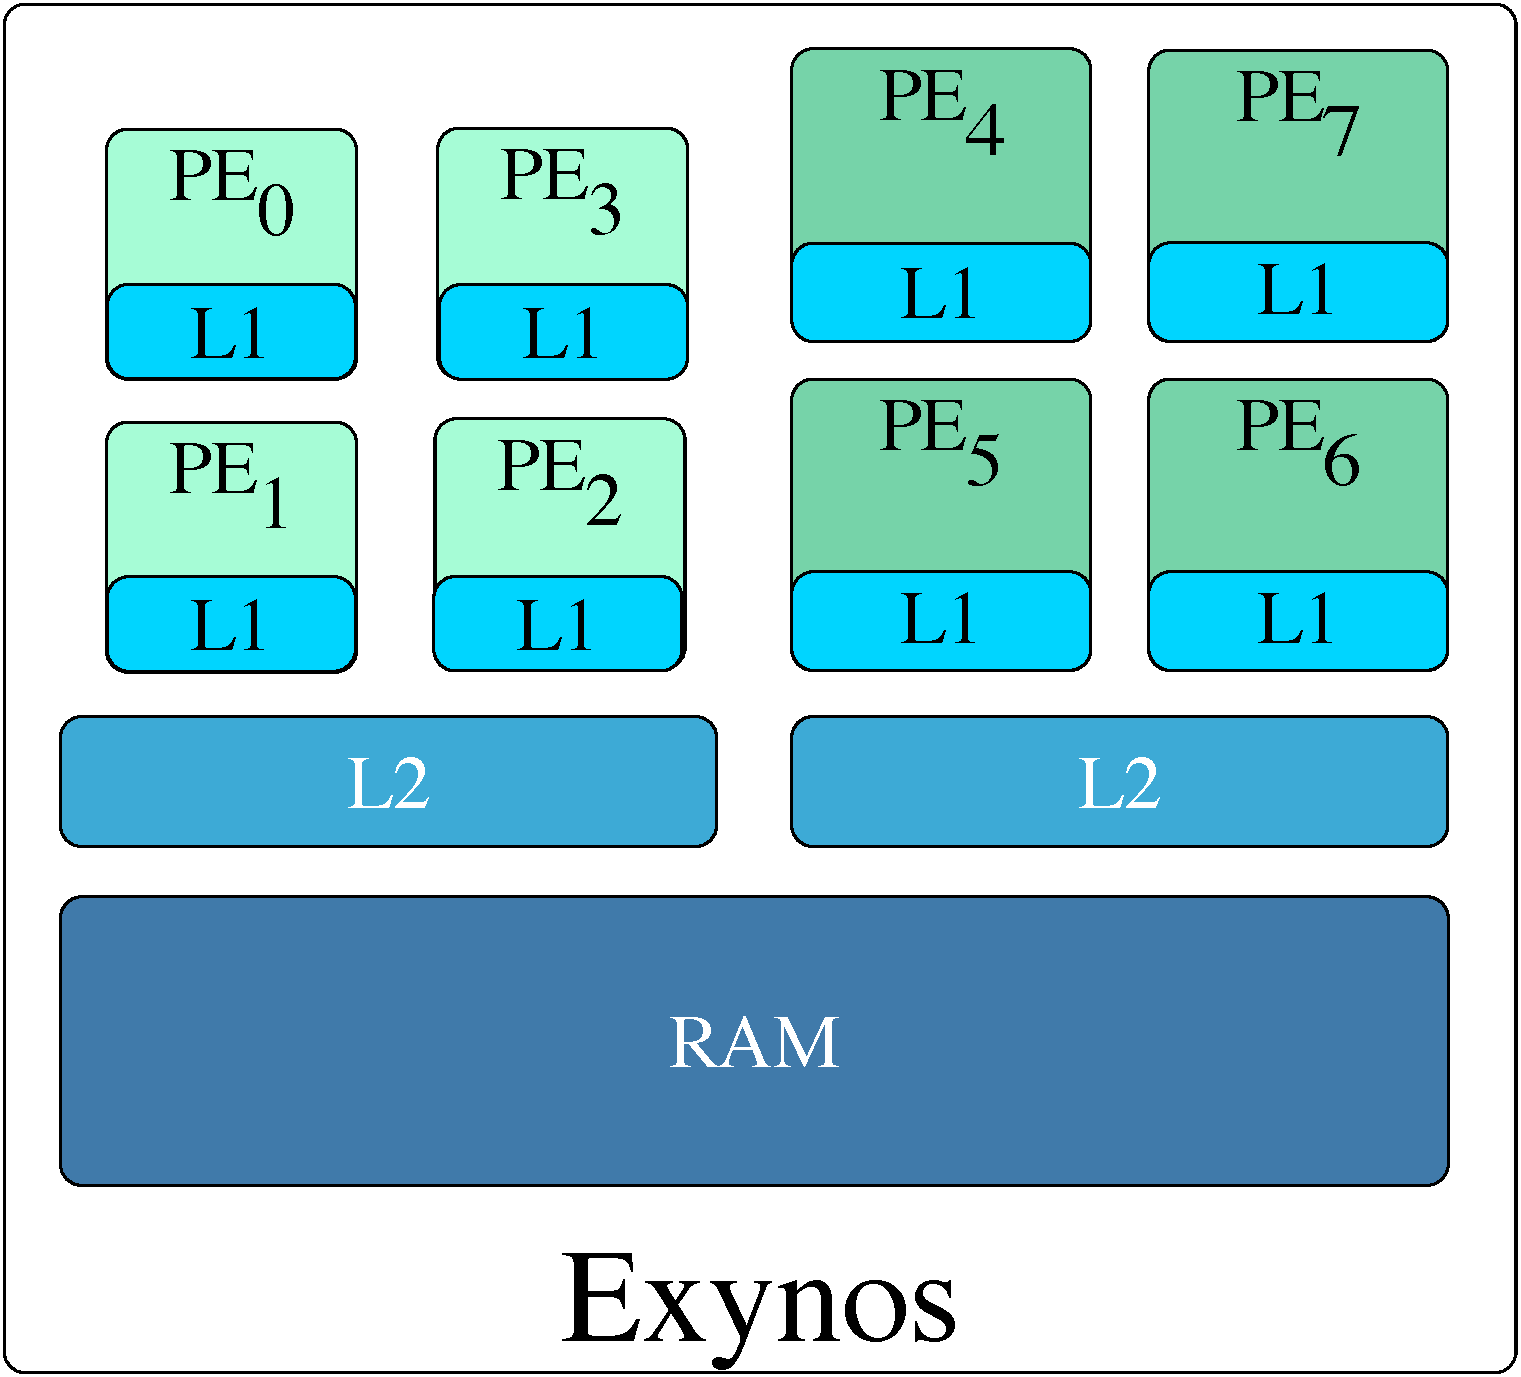
\includegraphics[width=0.255\textwidth]{figures/exynos.pdf}
	\caption{The heterogeneous Exynos architecture.}
	\label{fig:exynos}
%  \vspace{-3mm}
\end{figure}

\begin{figure}[t]
	\centering
	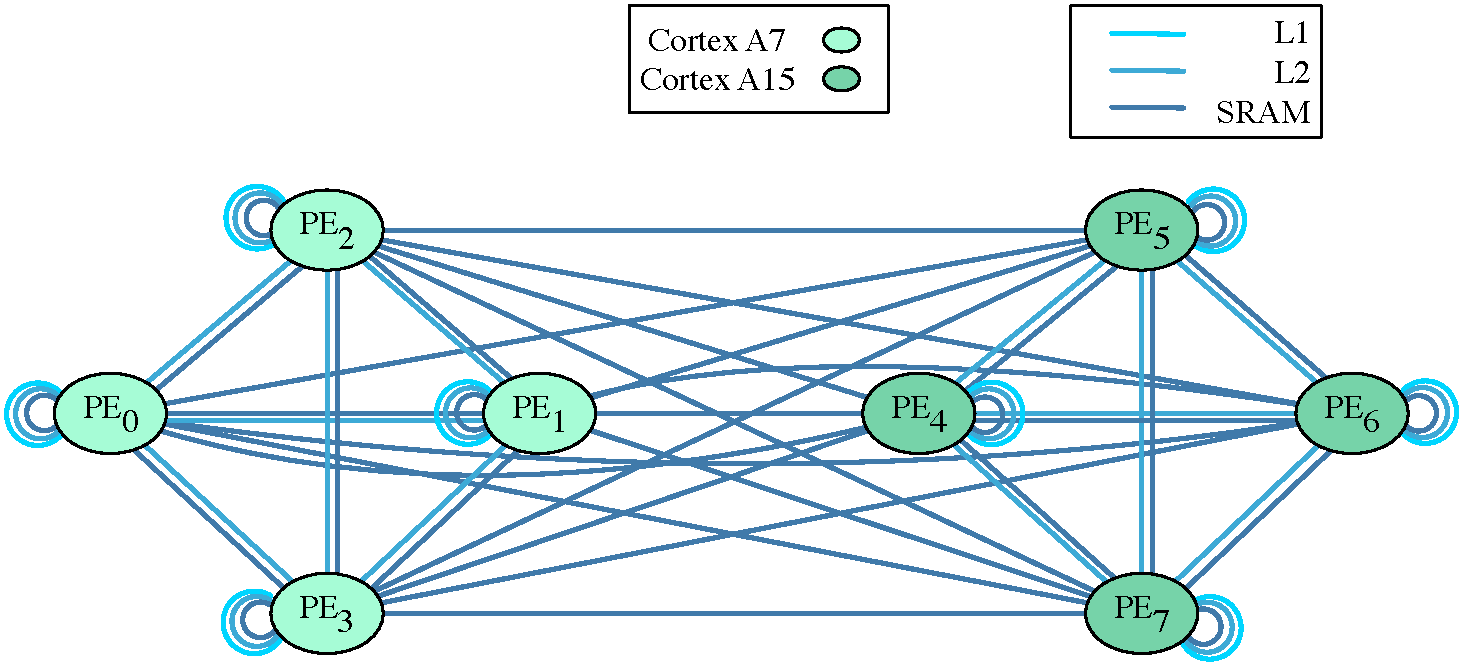
\includegraphics[width=0.5\textwidth]{figures/exynos_archgraph.pdf}
	\caption{The architecture graph of the Exynos.}
	\label{fig:arch_graph}
%  \vspace{-3mm}
\end{figure}

A mapping of a KPN $K$ to an architecture with architecture graph $A$ is thus simply a morphism of graphs $m: K \rightarrow A$. The condition that edges from $K$ are mapped to edges from $A$ ensures that FIFO buffers can be realized.
In practice, FIFO buffers and communication resources would have an annotation to their size, and a valid mapping would additional respect these sizing constraints. In this exposé, however, we will disregard these issues for simplicity.

An automorphism $\varphi: A \rightarrow A$ of the architecture graph, i.e. a graph isomorphism respecting labels of $A$ to itself, describes a symmetry of the problem.
Since even heterogenous architectures usually have several identical components, the groups of automorphisms of architecture graphs $A$ are non-trivial.
These symmetries of the architecture induce symmetries on mappings, as illustarted in Figure~\ref{fig:symmintro}.
\subsubsection{Reducing design-space exploration}

\subsubsection{Run-time adaptivity}

\subsection{Mapping Algorithms}
\subsubsection{Comparing Algorithms}
%The need for abstract models of architecture
%Metaheuristics > Heuristics, problem: time!
\subsubsection{Design centering}
 %Robust mappings

\section{Planned Work}

\subsection{Application Graphs}
\subsubsection{Graph transformations}
\"Yauhau

\subsubsection{Graph semantics}
The MacQueen Gap

\subsection{Architectures}

\subsubsection{Formal models of architecture}

\subsubsection{Symmetries}


\subsection{Traces}
%Motivation: dynamic behavior

\subsubsection{Mazurkiewicz Traces}

\subsubsection{Multiple Traces}

\subsubsection{Trace Compaction}
%Generatable by application -> small space

\subsubsection{Synthetic Traces}
Similar to compaction, 

\subsection{Mapping Algorithms}

\subsubsection{Genetic Algorithms}
%Structure: 

\subsubsection{Discrete Design Centering} 

\subsubsection{Compact Mappings}

\section{Timetable/Workplan}

\section{Related Work}
\section{Conclusions} 
%\bibliographystyle{ACM-Reference-Format}
\bibliographystyle{abbrv}
\bibliography{expose} 
\end{document}
